\section{Scanarea retelelor Wi-Fi}
\subsection{Scanare}
Pentru a scana punctele de access Wi-Fi la care dispozitivului se poate conecta ne trebuie o referinta la WiFi manager ca si in cazul afisarii informatiilor despre retea.
Vom face scanarea in functia onCreate a fragmetului, adaugand:

\begin{lstlisting}[language=Kotlin]
    val wifiManager = this.context?.getSystemService(Context.WIFI_SERVICE) as WifiManager;
    if (!wifiManager.startScan())
    {
        Log.e("WIFI", "FAILED TO START SCAN OF WIFI APs")
    }
\end{lstlisting}

Pentru a citi rezultatul scanarii trebuie sa folosim un receiver pentru evenimente de
tipul \textit{SCAN\_RESULTS\_AVAILABLE\_ACTION} produse de serviciul de sistem WiFi.

\begin{lstlisting}[language=Kotlin]
    val intentFilter = IntentFilter()
    intentFilter.addAction(WifiManager.SCAN_RESULTS_AVAILABLE_ACTION)
    this.activity?.registerReceiver(wifiScanReceiver, intentFilter)
\end{lstlisting}

Proprietatea wifiScanReceiver este un obiect de tipul \textit{BroadcastReceiver} care va fi definit in fragment.
Trebuie sa suprascriem metoda \texttt{onReceive} pentru a procesa rezultatele scanarii.
Pentru a updata modelul am adaugat si functia \texttt{onScanUpdate} in ViewModel.

\begin{lstlisting}[language=Kotlin]
    private val wifiScanReceiver = object : BroadcastReceiver() {
        override fun onReceive(context: Context, intent: Intent) {
            val success = intent.getBooleanExtra(WifiManager.EXTRA_RESULTS_UPDATED, false)
            if (success) {
                scanSuccess(context)
            } else {
                scanFailure(context)
            }
        }
    }
    @SuppressLint("MissingPermission")
    private fun scanSuccess(context: Context) {
        val wifiManager = context.getSystemService(Context.WIFI_SERVICE) as WifiManager
        val dashboardViewModel =
            ViewModelProvider(this)[DashboardViewModel::class.java]
        val results = wifiManager.scanResults
        dashboardViewModel.onScanUpdate(results)

        Log.i("WIFI", results.toString())
    }

    @SuppressLint("MissingPermission")
    private fun scanFailure(context: Context) {
        val wifiManager = context.getSystemService(Context.WIFI_SERVICE) as WifiManager
        val results = wifiManager.scanResults
        Log.i("WIFI", results.toString())
    }
\end{lstlisting}
\subsection{Afisarea rezultatelor}
Pentru a afisa in interfata grafica rezultatele scanarii trebuie sa folosim un element grafic.
In fragmentul {WifiScan} trebuie sa adaugam un element de tipul \texttt{RecyclerView}:
\begin{lstlisting}[language=XML]
<androidx.constraintlayout.widget.ConstraintLayout xmlns:android="http://schemas.android.com/apk/res/android"
    xmlns:app="http://schemas.android.com/apk/res-auto"
    xmlns:tools="http://schemas.android.com/tools"
    android:layout_width="match_parent"
    android:layout_height="match_parent"
    tools:context=".ui.dashboard.WiFiScanFragment">
    ...
    <androidx.recyclerview.widget.RecyclerView
        android:id="@+id/recyclerView"
        android:layout_width="0dp"
        android:layout_height="0dp"
        android:layout_marginStart="1dp"
        android:layout_marginTop="64dp"
        android:layout_marginEnd="1dp"
        android:layout_marginBottom="50dp"
        app:layout_constraintBottom_toBottomOf="parent"
        app:layout_constraintEnd_toEndOf="parent"
        app:layout_constraintHorizontal_bias="0.0"
        app:layout_constraintStart_toStartOf="parent"
        app:layout_constraintTop_toTopOf="parent"
        app:layout_constraintVertical_bias="0.0" />
</androidx.constraintlayout.widget.ConstraintLayout>
\end{lstlisting}
Pentru a putea transmite datele catre RecyclerView trebuie sa folosim un adaptor si un model pentru un element.
Modelul este o clasa data simpla care contine doar un string:
\begin{lstlisting}[language=Kotlin]
    data class NetworkItemViewModel(val name: String){

    }
\end{lstlisting}
Pentru a folosi RecyclerView trebuie sa definim un element grafic pentru un element din lista.
Acest element grafic este definit intr-un fisier XML separat.
\begin{lstlisting}[language=XML]
<?xml version="1.0" encoding="utf-8"?>
<androidx.cardview.widget.CardView xmlns:android="http://schemas.android.com/apk/res/android"
    android:layout_width="match_parent"
    android:layout_height="50dp"
    android:layout_margin="10dp"
    app:cardElevation="6dp"
    android:layout_marginHorizontal="10dp"
    android:layout_marginVertical="10dp"
    xmlns:app="http://schemas.android.com/apk/res-auto"
    xmlns:tools="http://schemas.android.com/tools"
    >

    <androidx.constraintlayout.widget.ConstraintLayout
        android:layout_width="match_parent"
        android:layout_height="wrap_content">

        <ImageView
            android:layout_width="60dp"
            android:layout_height="60dp"
            android:id="@+id/image"
            android:layout_marginStart="20dp"
            android:padding="8dp"
            android:adjustViewBounds="true"
            android:scaleType="fitXY"
            app:layout_constraintStart_toStartOf="parent"
            app:layout_constraintBottom_toBottomOf="parent"
            app:layout_constraintTop_toTopOf="parent"
            android:src="@drawable/ic_home_black_24dp"
            android:contentDescription="TODO" />
        <TextView
            android:layout_width="wrap_content"
            android:layout_height="wrap_content"
            android:id="@+id/network_name"
            android:textColor="@color/black"
            android:textSize="16sp"
            android:text="Title"
            android:layout_marginStart="20dp"
            app:layout_constraintStart_toEndOf="@id/image"
            app:layout_constraintTop_toTopOf="parent"
            app:layout_constraintBottom_toBottomOf="parent" />
    </androidx.constraintlayout.widget.ConstraintLayout>

</androidx.cardview.widget.CardView>

\end{lstlisting}
Clasa adaptor este o clasa care extinde RecyclerView. Adapter si care primeste ca parametru un ViewHolder.
ViewHolder este o clasa folosita pentru a seta proprietatile elementului grafic cu datele din obiectul de la pozitia corespunzatoare.

\begin{lstlisting}[language=Kotlin]
class NetworkItemAdapter(private val dataList: ArrayList<NetworkItemViewModel>):
    RecyclerView.Adapter<NetworkItemAdapter.ViewHolderClass>() {
    class ViewHolderClass(itemView: View): RecyclerView.ViewHolder(itemView) {
        val nameText: TextView = itemView.findViewById(R.id.network_name)
    }

    override fun onCreateViewHolder(parent: ViewGroup, viewType: Int): ViewHolderClass {
        val view = LayoutInflater.from(parent.context)
            .inflate(R.layout.network_item, parent, false)

        return ViewHolderClass(view)
    }

    override fun getItemCount(): Int {
      return dataList.size
    }

    override fun onBindViewHolder(holder: ViewHolderClass, position: Int) {
        val itemViewModel = dataList[position]
        holder.nameText.text = itemViewModel.name
    }
}
\end{lstlisting}

Acum ca avem dataele si elemetele necesare pentru a afisa rezultatele scanarii, trebuie sa le combinam, vom incepe in clasa de viewmodel, unde vom
adauga lista de retele scanate si o functie care va fi apelata de catre fragment pentru a updata lista.
\begin{lstlisting}
    class WiFiScanViewModel : ViewModel() {

    ...
    private val _scanResults = MutableLiveData<List<ScanResult>>().apply {
        value = ArrayList()
    }
    val scanResults: LiveData<List<ScanResult>> = _scanResults

    fun onScanUpdate(results: MutableList<ScanResult>)
    {
        _scanResults.value = results
    }

\end{lstlisting}

Iar cand view-ul fragmentului este creat, trebuie sa adaugam adaptorul si sa setam datele pentru RecyclerView.
\begin{lstlisting}[language=Kotlin]
    dashboardViewModel.scanResults.observe(viewLifecycleOwner) {
    val data = ArrayList<NetworkItemViewModel>()
    for (i in it)
    {
        data.add(NetworkItemViewModel(i.SSID))
    }
    val adapter = NetworkItemAdapter(data)
    binding.recyclerView.layoutManager = LinearLayoutManager(this.context)
    binding.recyclerView.adapter = adapter
\end{lstlisting}

Acum putem rula aplicatia si putem observa retelele Wi-Fi la care dispozitivul se poate conecta.

\begin{figure}[H]
    \centering
    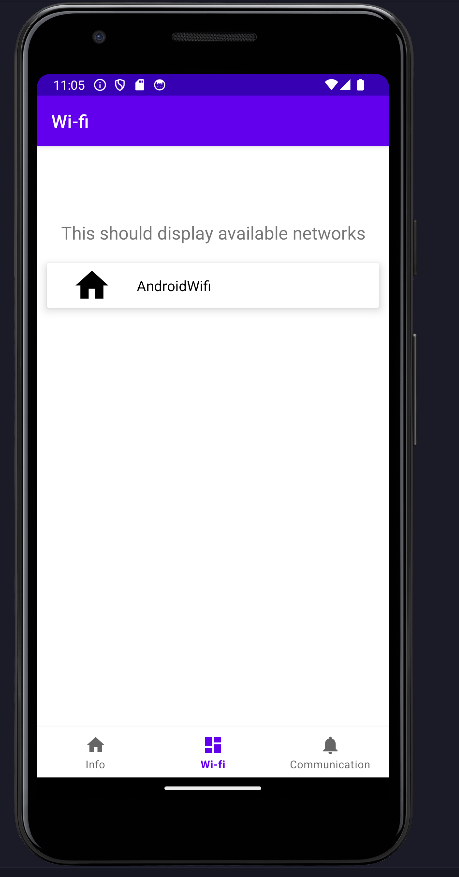
\includegraphics[width=0.7\linewidth]{figs/wifi_scan_res.png}
    \caption{Rezultatele scanarii retelelor Wi-Fi}
    \label{fig:wifi_scan_res}
\end{figure}